\documentclass{sig-alternate}
%\documentclass[a4paper,10pt]{article}
\usepackage[utf8]{inputenc}
%El template pincha con spanish babel
%\usepackage[spanish]{babel}
\usepackage{graphicx}
\usepackage{fancybox}
\usepackage[table]{xcolor}
\usepackage{soul}

\title{Controlando un sistema de producción de bienes} 

\numberofauthors{4}
\author{
\alignauthor
Pose, Alberto Miguel\\
       \affaddr{Instituto Tecnológico de Buenos Aires}\\
       \affaddr{Buenos Aires, Argentina}\\
       \email{apose@alu.itba.edu.ar}
\alignauthor
Catalano, Juan Ignacio\\
       \affaddr{Instituto Tecnológico de Buenos Aires}\\
       \affaddr{Buenos Aires, Argentina}\\
       \email{jcatalan@alu.itba.edu.ar}
\and
\alignauthor 
Palombo, Martín\\
       \affaddr{Instituto Tecnológico de Buenos Aires}\\
       \affaddr{Buenos Aires, Argentina}\\
       \email{mpalombo@alu.itba.edu.ar}
\alignauthor 
Vázquez, Santiago José\\
       \affaddr{Instituto Tecnológico de Buenos Aires}\\
       \affaddr{Buenos Aires, Argentina}\\
       \email{savazque@alu.itba.edu.ar}
}

\date{}




\begin{document}
\maketitle

\begin{abstract}
Se estudia el comportamiento del sistema correspondiente al inventario de producción de una empresa. Se plantean los modelos a lazo abierto y
lazo cerrado y se estudian condiciones de estabilidad de los mismos. Además se propone una adaptación para controlar la variación de la tasa
de ventas.
\end{abstract}

\section{Introducción}
\label{intro_section}
En nuestro país las huelgas a empresas se realizan median\-te el cese de las actividades de los empleados en protesta. Por otro
lado, se observa que las huelgas en países como Japón, vemos que son totalmente contrarias a las que estamos acostumbrados. Los obreros o empleados
en lugar de suspender su actividad, sobreproducen. Esto genera un exceso de inventario en los depósitos que se torna imposible de almacenar,
resultando en una pérdida mayor para la empresa. La importancia del control de productos en inventario se manifiesta en este
ejemplo y es nuestra motivación principal en el estudio de este tipo de sistemas. Un antecedente a este trabajo es el realizado por I. Luciani, J. Barreira y
F. Siviero titulado ``Sistema de Control de Inventario''\cite{iluciani}.\\ 
En la sección \ref{model_section} se presenta el modelo base (a lazo abierto) utilizado para realizar la simulación inicial. En la sección \ref{inventary_control_section} 
presenta una alternativa (a lazo cerrado), agregando un set de referencia para controlar la cantidad de productos en inventario. En la sección 
\ref{salesrate_control_section} se controla la tasa de ventas y se analizan los resultados obtenidos de realizar la simulación con dicho 
control. En la sección \ref{results_and_conclusions_section} se presentan los resultados y conclusiones obtenidas en todo el análisis 
realizado para este artículo.

\section{Modelo base}
\label{model_section}

Para nuestro análisis se considera una empresa que vende productos manufacturados los cuales son almacenados en un depósito.
El inventario de dichos bienes sigue una dinámica que cumple las siguientes propiedades:
\begin{enumerate}
\item Los productos son homogéneos. Esto permite poder realizar un mismo proceso para todos ellos.
\item La cantidad de productos manipulada en cada ejercicio es muy grande. Esta condición nos permite aproximar como continuo, este sistema de
naturaleza discreta.
\end{enumerate}
El modelo que se propone define $x_{1}(t)$ como el nivel
de inventario y $x_{2}(t)$ como la tasa de ventas del producto. Además,
se establece la velocidad de variación de la tasa de ventas como proporcional a $u(t)$, el flujo de entrada. Dicha relación queda explicitada en
\eqref{eq:la_k}.

\begin{equation}
\frac{dx_{2}}{dt}(t)=-Ku(t)\label{eq:la_k}\end{equation}


Donde K > 0.\\
Luego, definimos la velocidad de variación del inventario $\dot{x_{1}}(t)$ como se muestra en \eqref{eq:dotx1}.

\begin{equation}
\dot{x}_{1}(t)=u(t)-x_{2}(t)\label{eq:dotx1}\end{equation}

Esto significa que la variación de la cantidad de productos en inventario depende de lo
que se produce (entra) y de lo que se vende (sale). Este comportamiento se puede detallar como sigue:
\begin{enumerate}
\item Si $x_{2}<u(t)$ el nivel de inventario aumenta, $\dot{x}_{1}(t)>0$.
Esto se debe a que se produce más de lo que se vende.
\item Mientras que cuando $x_{2}(t)>u(t)$ el inventario disminuye más rápidamente que lo que se repone mediante nueva producción, 
$\dot{x}_{1}(t)<0$. Es decir, se vende más de lo que se produce.
\item Cuando $x_{2}=u(t)$, refleja que $\dot{x}_{1}(t)=0$ y la cantidad de
elementos en el inventario permanece constante. Esto puede atribuirse
a que se vende tanto como lo que se produce o a que no se vende ni
se produce ningún producto.

\end{enumerate}

Para realizar la simulación, consideramos $x_{2} = C$, una constante. Es decir, asumiendo que la tasa de ventas es invariante en el tiempo.\\
El modelo planteado en esta sección se denomina a lazo abierto, ya que no se propone realimentación alguna para la entrada del sistema. 
En la figura \ref{fig:lazo_abierto} podemos observar como evoluciona en este caso la cantidad de productos para el modelo a lazo abierto. 
Se puede notar un crecimiento indefinido de la cantidad de productos manufacturados que se debe a que las ventas disminuyen con el tiempo pero la 
produccion es siempre constante. Si $u(t)=0$, las existencias disminuyen hasta llegar a cero, es decir, se vacía el depósito. 

\begin{figure}[h]
\begin{center}
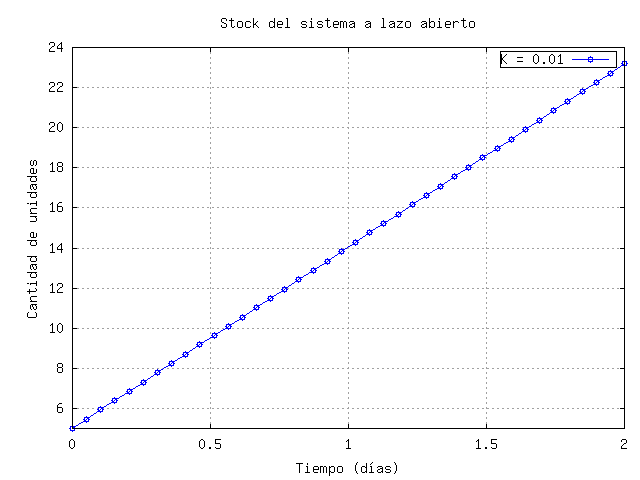
\includegraphics[width=8cm]{../src/lazo_abierto.png}
\caption{\label{fig:lazo_abierto}Cantidad de unidades almacenadas en función del tiempo. Simulación del modelo a lazo abierto.}
\end{center}
\end{figure}
Esto puede ser perjudicial para una compañia debido a los costos de almacenamiento junto a los costos de producción inmediatos de unidades 
que no se venden en el corto plazo. Más precisamente, como se puede ver en el sistema, no se venden nunca.\\
Si se observa la figura \ref{fig:lazo_abierto2} vemos que la tasa de ventas en este caso varía comportándose como una recta de pendiente negativa, 
es decir, que el sistema tiende a una situación en la cual no se vende nada, como se menciona anteriormente. Haciendo un análisis de los autovalores 
del sistema podemos ver que su parte real es cero y por ende el mismo es inestable. Si alcanza la estabilidad, es alrededor de un punto de equilibrio 
inestable, es decir que ante una pequeña perturbación pierde estabilidad y oscila. 

\begin{figure}[h]
\begin{center}
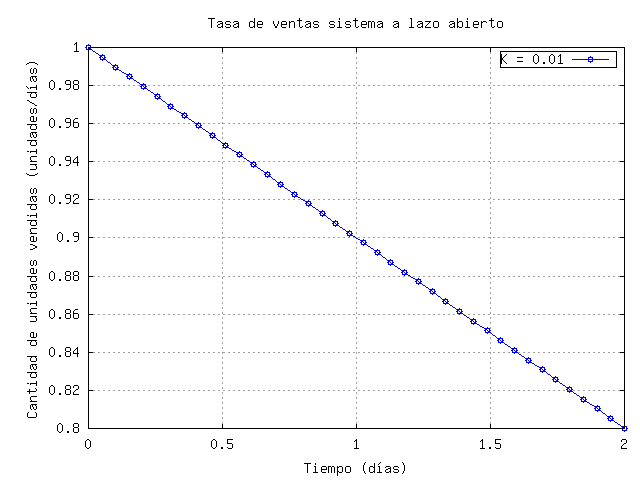
\includegraphics[width=8cm]{../src/lazo_abierto2.png}
\caption{\label{fig:lazo_abierto2} Tasa de ventas en función del tiempo. Simulación del modelo a lazo abierto.}
\end{center}
\end{figure}

\section{Controlando el inventario}
\label{inventary_control_section} 
Se desea controlar el nivel del inventario tomando como output $y(t)=x_{1}(t)$ y considerando
una función de referencia $r(t)$. Es decir, que $u(t)$ queda explicitado como se muestra en \eqref{eq:ut}.

\begin{equation}
u(t)= Ke(t) = K(r(t)-y(t))\label{eq:ut}\end{equation}
Resultando en la adaptación del modelo, ahora a lazo cerrado, que se muestra en \eqref{eq:lazo_cerrado}.

\begin{equation}
\dot{x}_1(t) = K(r(t) - x_{1}(t)) - C\label{eq:lazo_cerrado}\end{equation}

A fines de regular el inventario de manera tal que la cantidad de productos tienda a mantenerse constante, se define $r(t)$ como una función
constante.
Como se puede ver, esta adaptación del modelo queda completamente controlada por la constante $K$ definida en la sección anterior.  El valor alcanzado en el regimen estable
es el valor tomado como función (constante) de referencia, en nuestro caso $r(t) = 50$.\\
Podemos ver entonces que existe relación entre lo que se vende y lo que se produce y que dicha relación se encuentra gobernada por el valor de
$K$. La definición de dicho parámetro lleva a que el sistema sobreproduzca o no. Como podemos ver en la figura \ref{fig:lazo_cerrado_cant_unidades} para varios valores de $K$, 
el sistema se estabiliza en la cantidad de productos deseada. Sin embargo existe diferencia en el caso en el que $K$ tiende a cero, y en el que
tiende a aumentar. En el primer caso, el sistema se estabiliza en el valor prefijado como control del sistema. En el segundo caso, se llega a valores
menores de estabilidad. En la misma figura, podemos ver que para determinados valores de $K$ se dan situaciones que no son factibles en la realidad y que en el gráfico
se notan como las curvas que no alcanzan a estabilizarse en ningún valor.
\begin{figure}[h]
\begin{center}
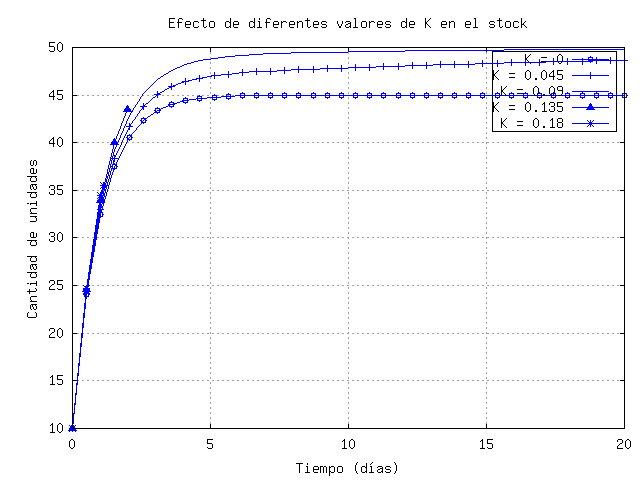
\includegraphics[width=8cm]{../src/k_plot.png}
\caption{\label{fig:lazo_cerrado_cant_unidades}Cantidad de productos en función del tiempo para distintos valores de $K$, simulando un sistema
a lazo cerrado.}
\end{center}
\end{figure}
Si se observa la figura \ref{fig:lazo_cerrado_var_tventas1} se puede apreciar como varía la tasa de ventas en este caso. Vemos que para los casos 
en que $K$ tiende a cero, la tasa de ventas se estabiliza, cada vez más a largo plazo, en cero.
% ver más jugos

\begin{figure}[h]
\begin{center}
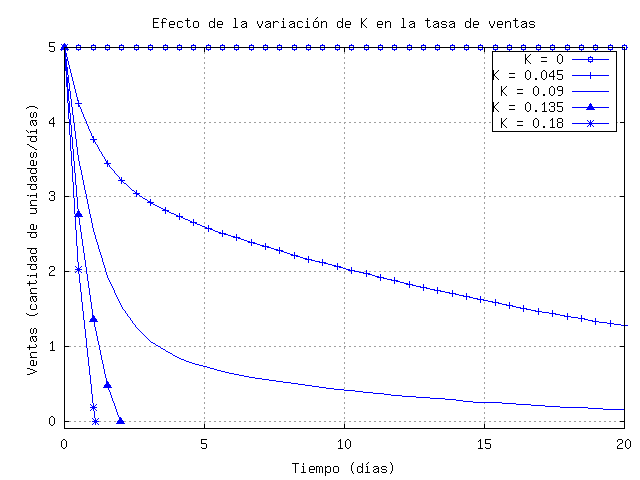
\includegraphics[width=8cm]{../src/k_plot3.png}
\caption{\label{fig:lazo_cerrado_var_tventas1}Tasa de ventas en función del tiempo para distintos valores de $K$, simulando un sistema
a lazo cerrado.}
\end{center}
\end{figure}

\section{Controlando la tasa de ventas}
\label{salesrate_control_section}
Veamos de plantear una adaptación del modelo en donde se controle el variación de la tasa de ventas. Para ello se propone una ecuación diferencial
tal que $\dot{x}_{2}$ dependa de la cantidad de productos en inventario. Esto se sustenta en la idea de que la variación de la tasa de unidades
vendidas depende de que se disponga de dichos bienes para su venta. Por ende, $\dot{x}_{2}$ resulta de la forma explicitada en \eqref{eq:x_2dot}.

\begin{equation}
 \label{eq:x_2dot}
 \frac{dx_{2}}{dt}(t) = 6x_1(t) - Ku(t)
\end{equation}
Como se puede ver, el comportamiento del modelo sigue regido por el valor de $K$. En la figura se observa que para determinados valores de $K$ el sistema
oscila inestablemente, mientras que para otros valores logra estabilizarse en el valor tomado como referencia. Empíricamente se muestra que cuando $0.799 < K < 5.687$ el modelo se comporta de forma estable. 
Es decir, se alcanza el comportamiento que se desea obtener mediante la regulación impuesta.\\
En la figura \ref{fig:lazo_cerrado_var_tventas2} vemos como para valores de $K$ fuera del rango de estabilidad, el modelo oscila de
forma inestable y si tomamos los valores dentro de dicho rango, el modelo se comporta de manera estable. Dentro de dicho rango, aumentar el 
valor de $K$ lleva a que el sistema se estabilice en valores mayores al utilizado como referencia. Por otro lado, si se utiliza un $K$ menor se puede ver como el 
modelo se estabiliza cada vez más cercano al establecido por la función de control.

\begin{figure}[h]
\begin{center}
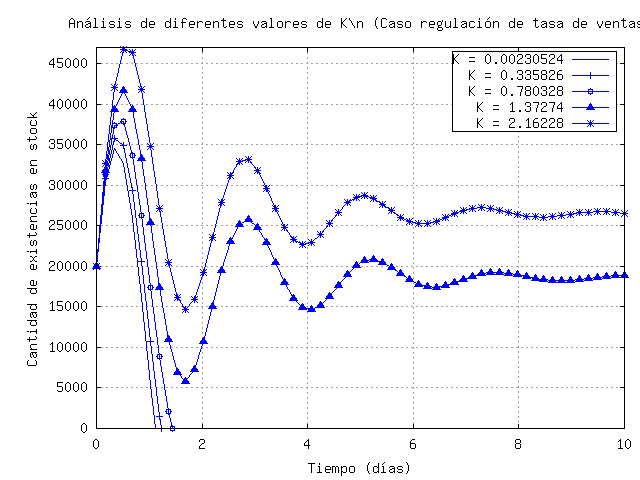
\includegraphics[width=8cm]{../src/k_plot2.png}
\caption{\label{fig:lazo_cerrado_var_tventas2}Cantidad de productos en función del tiempo para distintos valores de $K$, simulando un sistema
a lazo cerrado. Controlando la variación de la tasa de ventas.}
\end{center}
\end{figure}

\newpage

\section{Resultados y Conclusiones}
\label{results_and_conclusions_section}
A lo largo del trabajo se verifican los modelos tanto a lazo cerrado como lazo abierto. Se puede ver que el modelo planteado se adapta al comportamiento de un sistema de producción real. Al variar el inventario utilizando un modelo a lazo abierto observamos como la cantidad de productos aumenta de
forma lineal ya que las ventas disminuyen hasta ser nulas.  Por otro lado, en el modelo a lazo cerrado, se elige un subsistema de referencia.
Es decir, una función que controla las existencias en el inventario. En este caso vemos como la producción incrementa hasta llegar al valor 
que se fijó como referencia. En este caso el valor de $K$ también es fundamental ya que determina
en que cantidad de productos se estabiliza finalmente la producción. Para valores más cercanos a cero, se aproxima al punto
elegido como referencia. Al aumentarlo, el punto en el que se estabiliza disminuye. También, al controlar la variación de la tasa de ventas,
el valor de $K$ determina también la cantidad de productos en que se estabiliza el sistema.\\
Además, se ven oscilaciones en los primeros días de la simulación realizada controlando la variación de la tasa de ventas. Dichas oscilaciones
pueden también ser perjudiciales para un sistema de producción ya que pueden significar variaciones en los precios o en las cantidades importadas.\\
En la práctica, un empresario puede determinar aproximadamente el nivel de stock en el cual se 
estabilizará el sistema de producción. Esto puede permitir realizar conjeturas y tomar decisiones basándolas en los resultados de la simulación.
Por ejemplo, a partir de un posible aumento en los precios de los insumos el empresario puede querer afrontar la suba manteniendo el
mayor nivel de stock posible. 

\bibliographystyle{plain}
\nocite{*}
\bibliography{references}

\end{document}
